\subsubsection{Cơ sở dữ liệu -- PostgreSQL}
\label{subsubsec:co-so-du-lieu-postgresql}

Cơ sở dữ liệu của hệ thống dự kiến được thiết kế trên PostgreSQL, lưu trữ
tập trung dữ liệu phục vụ cả phân hệ quản trị viên và người sử dụng.
Thiết kế hướng đến việc đáp ứng các chức năng trong đề bài, hạn chế dữ liệu
trùng lặp và bảo đảm tính nhất quán giữa các thông tin có liên quan.

Các nhóm dữ liệu dự kiến gồm:

\begingroup
\small
\setlength{\tabcolsep}{4pt}
\begin{longtable}{|L{2cm}|L{4cm}|L{3cm}|L{\dimexpr\textwidth-9cm-8\tabcolsep-5\arrayrulewidth\relax}|}
  \caption{Các nhóm dữ liệu dự kiến và phạm vi thao tác}
  \label{tab:nhom-du-lieu-va-pham-vi}\\
  \hline
  \textbf{Nhóm dữ liệu} & \textbf{Nội dung dự kiến lưu trữ} &
  \textbf{Mục đích} & \textbf{Bên thao tác và phạm vi}\\
  \hline
  \endfirsthead
  \hline
  \textbf{Nhóm dữ liệu} & \textbf{Nội dung dự kiến lưu trữ} &
  \textbf{Mục đích} & \textbf{Bên thao tác và phạm vi}\\
  \hline
  \endhead
  Tài khoản &
  Tên đăng nhập, mật khẩu đã băm, hồ sơ cá nhân, quyền và trạng thái tài khoản &
  Phục vụ đăng nhập, phân quyền và quản lý người dùng &
  \textbf{User:} đăng ký, cập nhật hồ sơ và mật khẩu của mình.
  \textbf{Admin:} xem, thêm, cập nhật, xóa, khóa/mở khóa tài khoản và cập nhật
  mật khẩu theo quyền quản trị.\\
  \hline
  Quan hệ bạn bè &
  Yêu cầu kết bạn, trạng thái xử lý, quan hệ bạn bè và danh sách chặn &
  Phục vụ kết nối và quản lý quan hệ giữa người dùng &
  \textbf{User:} gửi, chấp nhận/từ chối yêu cầu, hủy kết bạn và chặn tài khoản.
  \textbf{Admin:} xem danh sách bạn bè và thống kê số lượng bạn bè.\\
  \hline
  Hội thoại và tin nhắn &
  Người tham gia, người gửi, nội dung và thời điểm gửi tin nhắn &
  Phục vụ chat, lưu lịch sử và truy xuất tin nhắn khi người nhận quay lại &
  \textbf{User:} gửi, xem, tìm kiếm và xóa lịch sử thuộc phạm vi được phép.
  \textbf{Backend:} kiểm tra quyền tham gia, lưu và chuyển tin nhắn.\\
  \hline
  Nhóm chat &
  Tên nhóm, thời điểm tạo, thành viên và quyền quản trị trong nhóm &
  Phục vụ quản lý và trao đổi tin nhắn theo nhóm &
  \textbf{User:} tạo nhóm và thực hiện các thao tác theo quyền.
  \textbf{Admin nhóm:} xóa thành viên theo quy định.
  \textbf{Admin hệ thống:} xem danh sách nhóm, thành viên và admin nhóm.\\
  \hline
  Báo cáo spam &
  Người báo cáo, tài khoản bị báo cáo, nội dung liên quan và thời điểm báo cáo &
  Hỗ trợ quản trị viên xem xét và xử lý &
  \textbf{User:} gửi báo cáo spam.
  \textbf{Admin:} xem, lọc, sắp xếp báo cáo và yêu cầu khóa tài khoản bị báo cáo.\\
  \hline
  Đăng nhập và hoạt động &
  Lịch sử đăng nhập, thời điểm mở ứng dụng và dữ liệu liên quan đến hoạt động chat &
  Phục vụ theo dõi và thống kê theo khoảng thời gian &
  \textbf{Backend:} ghi nhận dữ liệu từ các sự kiện của hệ thống.
  \textbf{Admin:} xem lịch sử, danh sách hoạt động và biểu đồ thống kê.\\
  \hline
\end{longtable}
\endgroup

``Bên thao tác'' chỉ chủ thể khởi tạo hoặc sử dụng chức năng. Mọi thao tác
đọc/ghi PostgreSQL đều được thực hiện qua backend sau khi kiểm tra quyền;
Admin và User không truy cập trực tiếp CSDL.

Các nhóm dữ liệu trên là cơ sở để xác định các bảng và mối quan hệ,
không mặc định mỗi nhóm tương ứng với một bảng. Thiết kế chi tiết sẽ xác định
khóa chính, khóa ngoại và các ràng buộc phù hợp để hạn chế bản ghi trùng lặp
hoặc tham chiếu không hợp lệ.

Đối với các thao tác làm thay đổi nhiều dữ liệu liên quan, nhóm dự kiến sử dụng
giao dịch để bảo đảm các thay đổi được thực hiện đồng bộ. Chẳng hạn, khi
chấp nhận yêu cầu kết bạn, việc cập nhật trạng thái yêu cầu và ghi nhận
quan hệ bạn bè cần được xử lý trong cùng một giao dịch.

Backend dự kiến truy cập PostgreSQL thông qua DAO và JDBC. Thông tin kết nối
được quản lý tại backend; Admin Client và User Client chỉ trao đổi yêu cầu,
kết quả với server qua socket TCP.

Thiết kế logic dưới đây cụ thể hóa các nhóm dữ liệu thành các thực thể,
thuộc tính, khóa và quan hệ dự kiến. Nội dung được dùng làm căn cứ xây dựng
script tạo CSDL trong V1; việc kết nối và xử lý dữ liệu từ ứng dụng thuộc
giai đoạn triển khai chức năng tiếp theo.

\paragraph{Sơ đồ quan hệ thực thể}
\mbox{}\par

ERD gồm 11 thực thể, chia thành các nhóm tài khoản, quan hệ bạn bè,
hội thoại và tin nhắn, báo cáo spam, đăng nhập và hoạt động.
\texttt{Conversation} được dùng chung cho hội thoại riêng và nhóm chat,
phân biệt bằng thuộc tính \texttt{type}. Thành viên và quyền trong từng
hội thoại được quản lý qua \texttt{ConversationMember}.

Hình~\ref{fig:erd-chatapp-v1} trình bày toàn bộ mô hình. Các thuộc tính
được mô tả lại trong Bảng~\ref{tab:tu-dien-du-lieu} để thuận tiện tra cứu.
Trong hình, PK là khóa chính, FK là khóa ngoại, UK là giá trị duy nhất;
dấu hỏi biểu thị thuộc tính có thể chưa có giá trị. Ký hiệu 1 và 0..N
thể hiện quan hệ một--nhiều, trong đó phía nhiều có thể chưa có bản ghi.

\begin{landscape}
\begin{figure}[p]
  \centering
  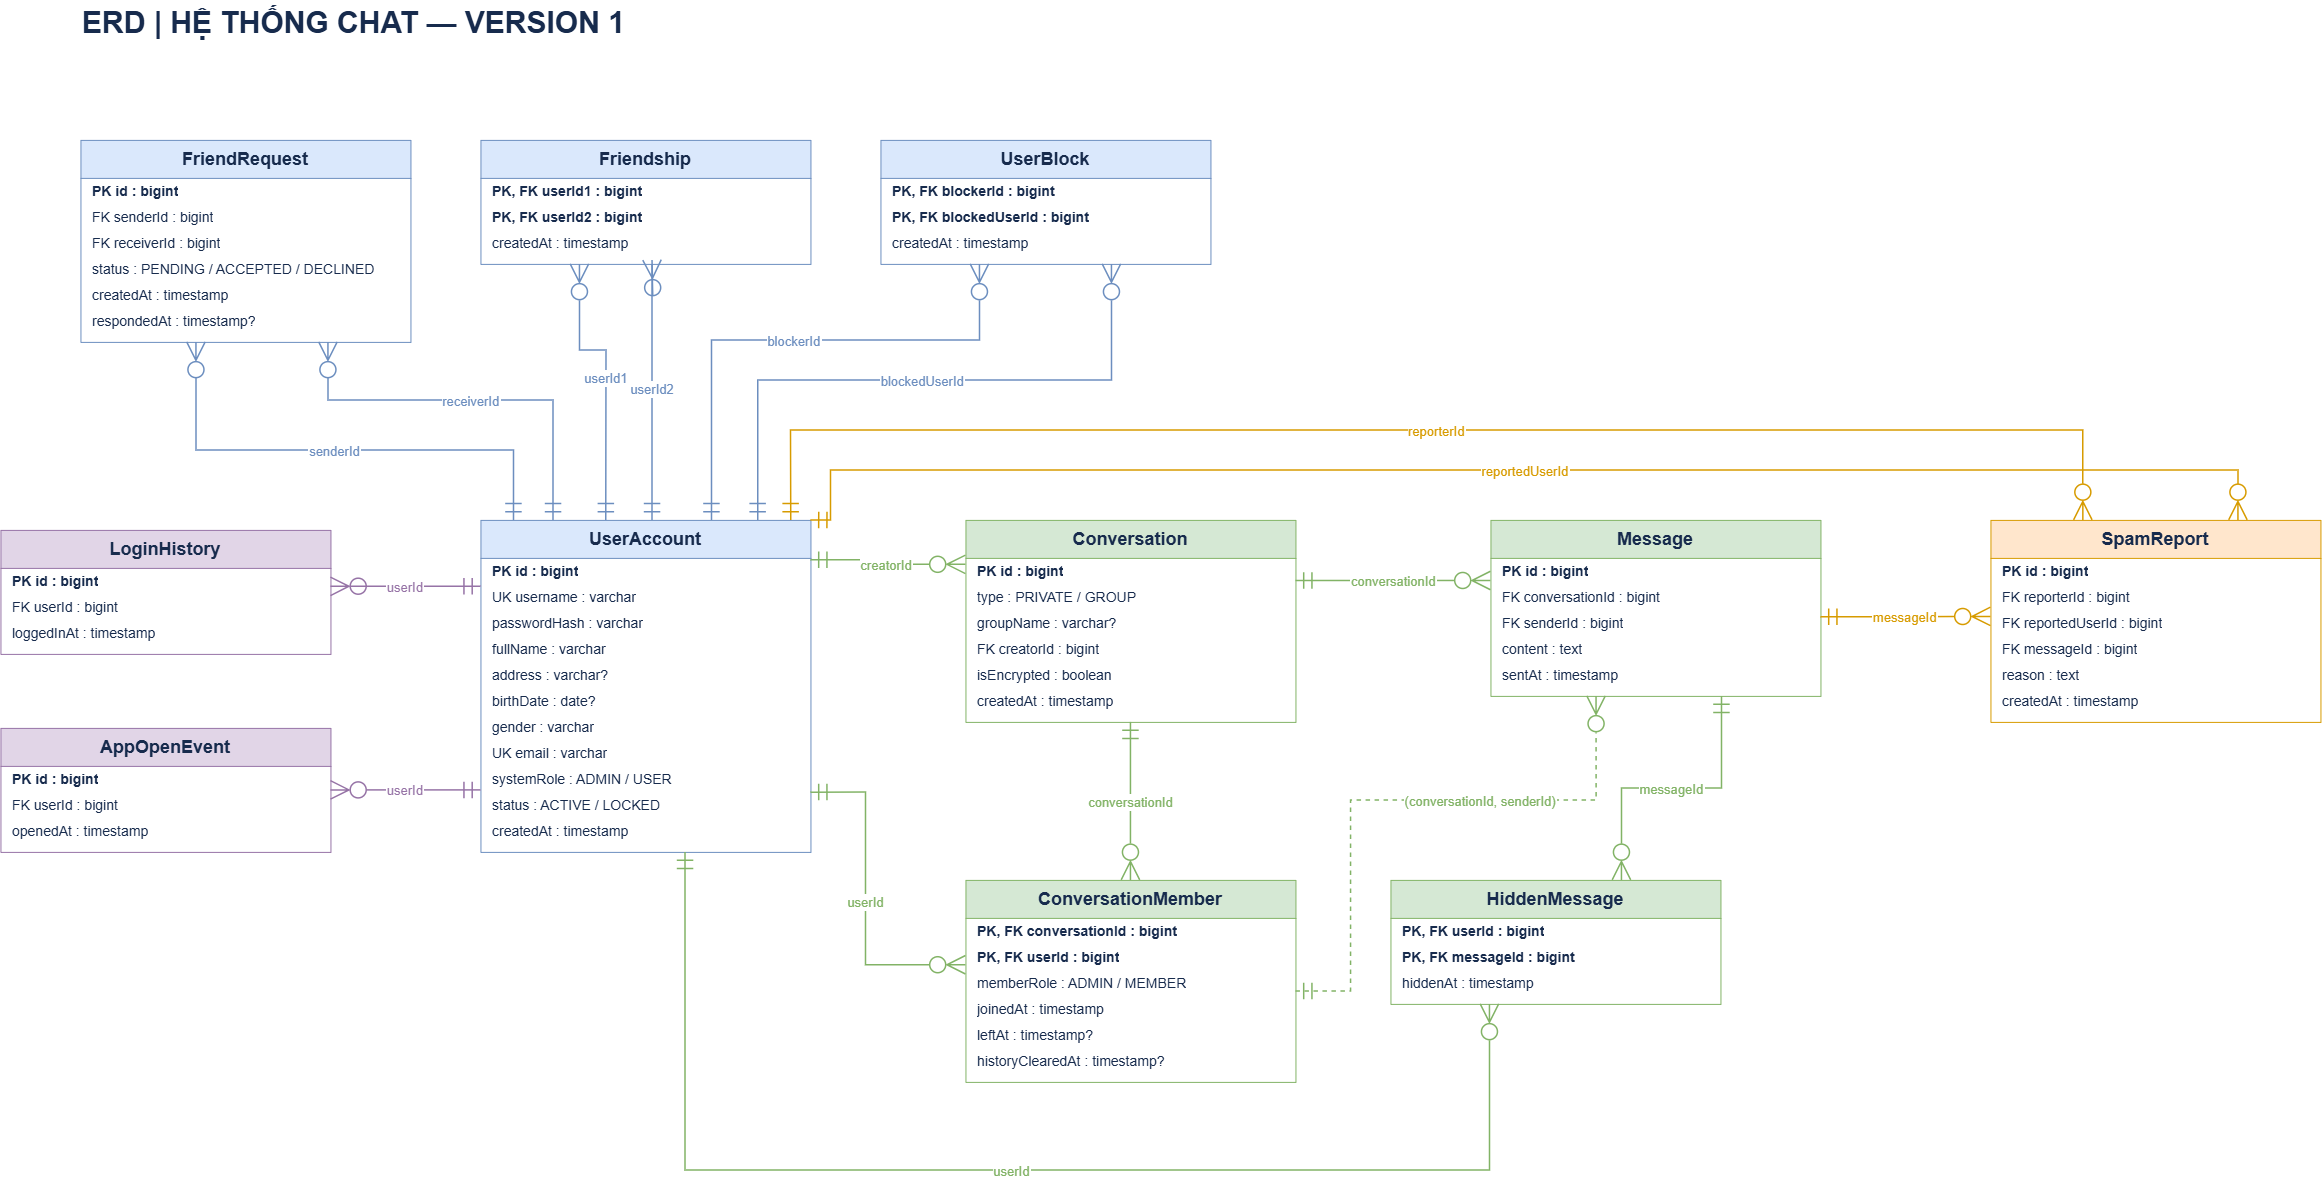
\includegraphics[width=\linewidth,height=0.83\textheight,keepaspectratio]{images/ERD-chatapp-v1.drawio.png}
  \caption{Sơ đồ quan hệ thực thể của hệ thống chat.}
  \label{fig:erd-chatapp-v1}
\end{figure}
\end{landscape}

Tên thực thể và tên thuộc tính trong phần mô tả được giữ thống nhất với
sơ đồ. Kiểu dữ liệu trong ERD được thể hiện ở mức logic; độ dài chuỗi,
giá trị mặc định và chính sách xử lý khi xóa dữ liệu cần được chốt khi
hoàn thiện script PostgreSQL.

\paragraph{Từ điển dữ liệu}
\mbox{}\par

Bảng dưới đây mô tả các thuộc tính của 11 thực thể trong ERD. Với khóa chính
kép, các thuộc tính có ký hiệu PK trong cùng thực thể cùng tạo thành một khóa;
không yêu cầu từng thuộc tính riêng lẻ là duy nhất. Các thuộc tính không có
dấu hỏi trong hình được dự kiến có giá trị; những trường có thể trống được
nêu riêng trong cột khóa và khả dụng.

\begingroup
\small
\setlength{\tabcolsep}{4pt}
\begin{longtable}{|L{3.6cm}|L{1.8cm}|L{2.9cm}|L{\dimexpr\textwidth-8.3cm-8\tabcolsep-5\arrayrulewidth\relax}|}
  \caption{Các thực thể và thuộc tính trong thiết kế CSDL}
  \label{tab:tu-dien-du-lieu}\\
  \hline
  \textbf{Thuộc tính} & \textbf{Kiểu logic} & \textbf{Khóa và khả dụng} & \textbf{Ý nghĩa}\\
  \hline
  \endfirsthead
  \hline
  \textbf{Thuộc tính} & \textbf{Kiểu logic} & \textbf{Khóa và khả dụng} & \textbf{Ý nghĩa}\\
  \hline
  \endhead
  \multicolumn{4}{|l|}{\textbf{UserAccount}}\\*
  \hline
  \texttt{id} & \texttt{bigint} & PK; Bắt buộc & Định danh tài khoản.\\
  \hline
  \texttt{username} & \texttt{varchar} & UK; Bắt buộc & Tên đăng nhập duy nhất; quy tắc chuẩn hóa chữ hoa/thường cần thống nhất khi tạo CSDL.\\
  \hline
  \texttt{passwordHash} & \texttt{varchar} & Bắt buộc & Giá trị băm mật khẩu; không lưu mật khẩu dạng văn bản rõ.\\
  \hline
  \texttt{fullName} & \texttt{varchar} & Bắt buộc & Họ tên của người dùng.\\
  \hline
  \texttt{address} & \texttt{varchar} & Có thể trống & Địa chỉ trong hồ sơ cá nhân.\\
  \hline
  \texttt{birthDate} & \texttt{date} & Có thể trống & Ngày sinh, tách biệt với các thời điểm ghi nhận hoạt động.\\
  \hline
  \texttt{gender} & \texttt{varchar} & Bắt buộc & Giới tính trong hồ sơ cá nhân.\\
  \hline
  \texttt{email} & \texttt{varchar} & UK; Bắt buộc & Email duy nhất, phục vụ liên hệ và khởi tạo lại mật khẩu.\\
  \hline
  \texttt{systemRole} & \texttt{varchar} & Bắt buộc & Quyền hệ thống: \texttt{ADMIN} hoặc \texttt{USER}.\\
  \hline
  \texttt{status} & \texttt{varchar} & Bắt buộc & Trạng thái tài khoản: \texttt{ACTIVE} hoặc \texttt{LOCKED}.\\
  \hline
  \texttt{createdAt} & \texttt{timestamp} & Bắt buộc & Thời điểm tạo tài khoản, phục vụ thống kê đăng ký mới.\\
  \hline
  \multicolumn{4}{|l|}{\textbf{FriendRequest}}\\*
  \hline
  \texttt{id} & \texttt{bigint} & PK; Bắt buộc & Định danh yêu cầu kết bạn.\\
  \hline
  \texttt{senderId} & \texttt{bigint} & FK; Bắt buộc & Tài khoản gửi yêu cầu, tham chiếu \texttt{UserAccount.id}.\\
  \hline
  \texttt{receiverId} & \texttt{bigint} & FK; Bắt buộc & Tài khoản nhận yêu cầu, tham chiếu \texttt{UserAccount.id}.\\
  \hline
  \texttt{status} & \texttt{varchar} & Bắt buộc & Trạng thái \texttt{PENDING}, \texttt{ACCEPTED} hoặc \texttt{DECLINED}.\\
  \hline
  \texttt{createdAt} & \texttt{timestamp} & Bắt buộc & Thời điểm gửi yêu cầu.\\
  \hline
  \texttt{respondedAt} & \texttt{timestamp} & Có thể trống & Thời điểm đồng ý hoặc từ chối; có thể trống khi đang chờ.\\
  \hline
  \multicolumn{4}{|l|}{\textbf{Friendship}}\\*
  \hline
  \texttt{userId1} & \texttt{bigint} & PK kép, FK; Bắt buộc & Tài khoản thứ nhất; tham chiếu \texttt{UserAccount.id}.\\
  \hline
  \texttt{userId2} & \texttt{bigint} & PK kép, FK; Bắt buộc & Tài khoản thứ hai; tham chiếu \texttt{UserAccount.id}.\\
  \hline
  \texttt{createdAt} & \texttt{timestamp} & Bắt buộc & Thời điểm xác lập quan hệ bạn bè.\\
  \hline
  \multicolumn{4}{|l|}{\textbf{UserBlock}}\\*
  \hline
  \texttt{blockerId} & \texttt{bigint} & PK kép, FK; Bắt buộc & Tài khoản chủ động chặn, tham chiếu \texttt{UserAccount.id}.\\
  \hline
  \texttt{blockedUserId} & \texttt{bigint} & PK kép, FK; Bắt buộc & Tài khoản bị chặn, tham chiếu \texttt{UserAccount.id}.\\
  \hline
  \texttt{createdAt} & \texttt{timestamp} & Bắt buộc & Thời điểm tạo quan hệ chặn.\\
  \hline
  \multicolumn{4}{|l|}{\textbf{Conversation}}\\*
  \hline
  \texttt{id} & \texttt{bigint} & PK; Bắt buộc & Định danh hội thoại.\\
  \hline
  \texttt{type} & \texttt{varchar} & Bắt buộc & Loại hội thoại: \texttt{PRIVATE} hoặc \texttt{GROUP}.\\
  \hline
  \texttt{groupName} & \texttt{varchar} & Có thể trống & Tên nhóm; không dùng cho hội thoại riêng.\\
  \hline
  \texttt{creatorId} & \texttt{bigint} & FK; Bắt buộc & Tài khoản tạo hội thoại, tham chiếu \texttt{UserAccount.id}.\\
  \hline
  \texttt{isEncrypted} & \texttt{boolean} & Bắt buộc & Cờ đánh dấu nhóm có sử dụng mã hóa; không thay thế dữ liệu quản lý khóa.\\
  \hline
  \texttt{createdAt} & \texttt{timestamp} & Bắt buộc & Thời điểm tạo hội thoại hoặc nhóm chat.\\
  \hline
  \multicolumn{4}{|l|}{\textbf{ConversationMember}}\\*
  \hline
  \texttt{conversationId} & \texttt{bigint} & PK kép, FK; Bắt buộc & Hội thoại tham gia, tham chiếu \texttt{Conversation.id}.\\
  \hline
  \texttt{userId} & \texttt{bigint} & PK kép, FK; Bắt buộc & Người tham gia, tham chiếu \texttt{UserAccount.id}.\\
  \hline
  \texttt{memberRole} & \texttt{varchar} & Bắt buộc & Quyền trong hội thoại: \texttt{ADMIN} hoặc \texttt{MEMBER}; khác quyền hệ thống.\\
  \hline
  \texttt{joinedAt} & \texttt{timestamp} & Bắt buộc & Thời điểm tham gia hội thoại.\\
  \hline
  \texttt{leftAt} & \texttt{timestamp} & Có thể trống & Thời điểm rời hoặc bị xóa khỏi nhóm; có thể trống khi còn tham gia.\\
  \hline
  \texttt{historyClearedAt} & \texttt{timestamp} & Có thể trống & Mốc ẩn toàn bộ lịch sử cũ đối với thành viên này, theo cách hiểu xóa riêng từng người.\\
  \hline
  \multicolumn{4}{|l|}{\textbf{Message}}\\*
  \hline
  \texttt{id} & \texttt{bigint} & PK; Bắt buộc & Định danh tin nhắn.\\
  \hline
  \texttt{conversationId} & \texttt{bigint} & FK; Bắt buộc & Hội thoại chứa tin, tham chiếu \texttt{Conversation.id}; đồng thời thuộc khóa ngoại kép của người gửi.\\
  \hline
  \texttt{senderId} & \texttt{bigint} & FK; Bắt buộc & Tài khoản gửi; cùng \texttt{conversationId} tham chiếu cặp khóa của \texttt{ConversationMember}.\\
  \hline
  \texttt{content} & \texttt{text} & Bắt buộc & Nội dung tin nhắn. Cách lưu nội dung mã hóa cần được thiết kế thêm.\\
  \hline
  \texttt{sentAt} & \texttt{timestamp} & Bắt buộc & Thời điểm gửi tin nhắn, dùng sắp xếp lịch sử và lọc theo thời gian.\\
  \hline
  \multicolumn{4}{|l|}{\textbf{HiddenMessage}}\\*
  \hline
  \texttt{userId} & \texttt{bigint} & PK kép, FK; Bắt buộc & Người ẩn tin nhắn, tham chiếu \texttt{UserAccount.id}.\\
  \hline
  \texttt{messageId} & \texttt{bigint} & PK kép, FK; Bắt buộc & Tin nhắn bị ẩn, tham chiếu \texttt{Message.id}.\\
  \hline
  \texttt{hiddenAt} & \texttt{timestamp} & Bắt buộc & Thời điểm người dùng ẩn tin khỏi lịch sử của mình.\\
  \hline
  \multicolumn{4}{|l|}{\textbf{SpamReport}}\\*
  \hline
  \texttt{id} & \texttt{bigint} & PK; Bắt buộc & Định danh báo cáo spam.\\
  \hline
  \texttt{reporterId} & \texttt{bigint} & FK; Bắt buộc & Tài khoản báo cáo, tham chiếu \texttt{UserAccount.id}.\\
  \hline
  \texttt{reportedUserId} & \texttt{bigint} & FK; Bắt buộc & Tài khoản bị báo cáo, tham chiếu \texttt{UserAccount.id}.\\
  \hline
  \texttt{messageId} & \texttt{bigint} & FK; Bắt buộc & Tin nhắn liên quan, tham chiếu \texttt{Message.id}.\\
  \hline
  \texttt{reason} & \texttt{text} & Bắt buộc & Lý do hoặc mô tả nội dung báo cáo.\\
  \hline
  \texttt{createdAt} & \texttt{timestamp} & Bắt buộc & Thời điểm gửi báo cáo, dùng để lọc và sắp xếp.\\
  \hline
  \multicolumn{4}{|l|}{\textbf{LoginHistory}}\\*
  \hline
  \texttt{id} & \texttt{bigint} & PK; Bắt buộc & Định danh lượt đăng nhập.\\
  \hline
  \texttt{userId} & \texttt{bigint} & FK; Bắt buộc & Tài khoản đăng nhập, tham chiếu \texttt{UserAccount.id}.\\
  \hline
  \texttt{loggedInAt} & \texttt{timestamp} & Bắt buộc & Thời điểm đăng nhập thành công.\\
  \hline
  \multicolumn{4}{|l|}{\textbf{AppOpenEvent}}\\*
  \hline
  \texttt{id} & \texttt{bigint} & PK; Bắt buộc & Định danh lượt mở ứng dụng.\\
  \hline
  \texttt{userId} & \texttt{bigint} & FK; Bắt buộc & Tài khoản được ghi nhận hoạt động, tham chiếu \texttt{UserAccount.id}.\\
  \hline
  \texttt{openedAt} & \texttt{timestamp} & Bắt buộc & Thời điểm mở ứng dụng, phục vụ thống kê lượt mở và người hoạt động.\\
  \hline
\end{longtable}
\endgroup

Các thuộc tính thời gian dùng để sắp xếp và thống kê cần được lưu, diễn giải
thống nhất về múi giờ khi tạo script và kết nối JDBC. Tên đăng nhập, email,
trạng thái tài khoản và trạng thái yêu cầu cũng cần có quy ước giá trị nhất quán.

\paragraph{Các quan hệ chính}
\mbox{}\par

Một tài khoản có thể gửi hoặc nhận nhiều yêu cầu kết bạn, xuất hiện trong
nhiều quan hệ bạn bè và quan hệ chặn, đồng thời tham gia nhiều hội thoại.
Với các quan hệ có hai vai trò, hai thuộc tính cùng tham chiếu đến
\texttt{UserAccount.id} nhưng có ý nghĩa khác nhau, chẳng hạn người gửi
và người nhận yêu cầu kết bạn.

\begin{itemize}
  \item \textbf{Tài khoản và quan hệ bạn bè:}
    \texttt{FriendRequest.senderId} và \texttt{receiverId},
    hai thuộc tính của khóa chính \texttt{Friendship},
    cùng \texttt{UserBlock.blockerId} và \texttt{blockedUserId}
    đều tham chiếu đến tài khoản tương ứng.
  \item \textbf{Tài khoản và hội thoại:}
    \texttt{Conversation.creatorId} tham chiếu người tạo.
    Quan hệ nhiều--nhiều giữa tài khoản và hội thoại được tách qua
    \texttt{ConversationMember}, có khóa chính kép
    \texttt{(conversationId, userId)}.
  \item \textbf{Hội thoại và tin nhắn:}
    mỗi tin nhắn thuộc một hội thoại. Cặp
    \texttt{(conversationId, senderId)} trong \texttt{Message}
    tham chiếu khóa chính của \texttt{ConversationMember}, giúp bảo đảm
    người gửi có bản ghi thành viên trong đúng hội thoại.
    Điều kiện còn đang tham gia tại thời điểm gửi cần được backend kiểm tra thêm.
  \item \textbf{Tin nhắn và lịch sử cá nhân:}
    \texttt{HiddenMessage} liên kết một người dùng với một tin nhắn.
    Khóa chính kép \texttt{(userId, messageId)} ngăn ghi nhận trùng
    cùng một lần ẩn tin của người dùng đó.
  \item \textbf{Tin nhắn và báo cáo spam:}
    \texttt{SpamReport} tham chiếu người báo cáo, tài khoản bị báo cáo
    và tin nhắn liên quan; một tin nhắn có thể xuất hiện trong nhiều báo cáo.
  \item \textbf{Tài khoản và hoạt động:}
    mỗi bản ghi \texttt{LoginHistory} hoặc \texttt{AppOpenEvent}
    thuộc một tài khoản; một tài khoản có thể có nhiều bản ghi theo thời gian.
\end{itemize}

\paragraph{Ràng buộc và quy tắc dữ liệu dự kiến}
\mbox{}\par

Các khóa chính, khóa ngoại và ràng buộc duy nhất được dự kiến thể hiện trong
CSDL. Những quy tắc liên quan đến quyền truy cập, trạng thái tham gia hoặc
thay đổi đồng thời nhiều bản ghi cần được kiểm tra thêm tại backend;
không xem các khóa trong ERD là đủ để thực hiện toàn bộ nghiệp vụ.

\begin{enumerate}
  \item \textbf{Tài khoản:} tên đăng nhập và email là duy nhất;
    mật khẩu được lưu dưới dạng đã băm. \texttt{systemRole} phân biệt
    Admin hệ thống với User; \texttt{status} phân biệt tài khoản đang hoạt động
    với tài khoản bị khóa.
  \item \textbf{Bạn bè và chặn:} hai người trong một quan hệ phải khác nhau.
    \texttt{Friendship} lưu cặp ID theo quy ước
    \texttt{userId1 < userId2}, kết hợp khóa chính kép để không lưu
    hai chiều của cùng một quan hệ. Quan hệ chặn có hướng nên A chặn B
    không đồng nghĩa B chặn A.
  \item \textbf{Hội thoại và thành viên:} \texttt{type} nhận
    \texttt{PRIVATE} hoặc \texttt{GROUP}; tên nhóm được dùng cho hội thoại nhóm.
    Hội thoại riêng có hai người tham gia; khi tạo nhóm cần người tạo và
    ít nhất một người dùng khác. Khóa chính kép của thành viên ngăn một
    người xuất hiện hai lần trong cùng hội thoại.
  \item \textbf{Quyền trong nhóm:} \texttt{memberRole} nhận
    \texttt{ADMIN} hoặc \texttt{MEMBER}, độc lập với quyền quản trị hệ thống.
    Chỉ admin nhóm được xóa thành viên theo yêu cầu đề bài.
    Khi gửi tin, backend cần kiểm tra trạng thái thành viên và quyền hiện tại.
  \item \textbf{Báo cáo spam:} người báo cáo phải có quyền xem nội dung
    liên quan; tin nhắn được báo cáo phải thuộc tài khoản bị báo cáo.
    Backend cần kiểm tra các điều kiện này ngoài việc kiểm tra các khóa ngoại.
  \item \textbf{Tính đồng bộ:} khi chấp nhận kết bạn, cập nhật yêu cầu và tạo
    quan hệ bạn bè trong cùng giao dịch. Khi chặn và hủy kết bạn, các thay đổi
    liên quan cũng cần được xử lý đồng bộ để tránh trạng thái mâu thuẫn.
\end{enumerate}

\paragraph{Xóa lịch sử và mã hóa nhóm}
\mbox{}\par

Thiết kế đề xuất hiểu thao tác xóa lịch sử là xóa khỏi phía người thực hiện.
\texttt{HiddenMessage} ghi nhận việc ẩn từng tin nhắn;
\texttt{ConversationMember.historyClearedAt} xác định mốc xóa toàn bộ lịch sử
cũ của thành viên. Khi truy xuất, các tin đã ẩn và tin trước mốc này
không được hiển thị cho người đó; lịch sử của người tham gia khác không
tự động bị xóa. Đây là cách hiểu cần nhóm thống nhất khi chốt thiết kế.

Thuộc tính \texttt{Conversation.isEncrypted} chỉ ghi nhận trạng thái mã hóa
của nhóm. ERD hiện tại chưa mô tả chi tiết dữ liệu phục vụ quản lý khóa,
thay đổi khóa hoặc định dạng nội dung mã hóa; cần hoàn thiện phần này trước
khi khẳng định thiết kế dữ liệu đã đáp ứng đầy đủ chức năng mã hóa nhóm.
Tương tự, chính sách giữ lại hoặc xử lý dữ liệu liên quan khi xóa tài khoản
cần được xác định trước khi chốt các hành vi của khóa ngoại trong script.

\paragraph{Dữ liệu phục vụ thống kê}
\mbox{}\par

Mô hình không tạo bảng thống kê riêng khi số liệu có thể được tính từ
các dữ liệu gốc. Các chức năng của Admin được đối chiếu như sau:

\begin{itemize}
  \item \hyperlink{F14}{F14}: lấy các lượt đăng nhập từ
    \texttt{LoginHistory}, kết hợp hồ sơ tài khoản và sắp xếp theo thời gian.
  \item \hyperlink{F17}{F17}--\hyperlink{F18}{F18}: lọc
    \texttt{UserAccount.createdAt} theo năm đã chọn; tổng hợp số tài khoản
    tạo mới theo tháng của năm được chọn.
  \item \hyperlink{F19}{F19}: đếm quan hệ trong \texttt{Friendship};
    \textbf{Total network} là hợp của tập bạn trực tiếp và tập bạn của bạn,
    loại chính tài khoản đang xét và chỉ đếm mỗi tài khoản một lần.
    \textbf{Friends of friends only} loại thêm các bạn trực tiếp; người bạn
    chung được xác định từ hai quan hệ bạn bè nối tiếp nhau.
  \item \hyperlink{F20}{F20}: đếm lượt mở ứng dụng từ
    \texttt{AppOpenEvent}; đối chiếu tin nhắn, hội thoại và thành viên để
    xác định số người và số nhóm có trao đổi trong năm đã chọn.
  \item \hyperlink{F21}{F21}: đếm các tài khoản khác nhau có mở ứng dụng
    trong từng tháng, không dùng tổng số lượt mở thay cho số người hoạt động.
\end{itemize}

Lịch sử đăng nhập và lượt mở ứng dụng được tách riêng vì việc mở lại ứng dụng
không nhất thiết là một lần đăng nhập mới. Trạng thái online/offline sẽ cần
được backend xác định từ kết nối thực tế khi triển khai; một bản ghi đăng nhập
cũ không đủ chứng minh người dùng đang online.

Bộ chọn \textbf{Period} áp dụng cùng một năm dương lịch cho các bảng và biểu đồ.
Truy vấn theo năm bao gồm các mốc từ đầu năm đến trước đầu năm kế tiếp theo
múi giờ thống nhất của hệ thống. Biểu đồ luôn có 12 tháng; tổng
\textbf{Active users} của cả năm đếm mỗi tài khoản một lần, kể cả khi tài khoản
có hoạt động trong nhiều tháng.

\paragraph{Dữ liệu cho phần mở rộng quản trị}
\mbox{}\par
ERD hiện tại hỗ trợ trạng thái \texttt{ACTIVE}/\texttt{LOCKED} và các báo cáo
spam. Nhật ký khóa/mở khóa trong nguyên mẫu là phần mở rộng cần lưu thời điểm,
tài khoản bị tác động và quản trị viên thực hiện. Nhật ký hoạt động nhóm có thể
lấy mốc gửi tin nhắn và tham gia/rời nhóm từ các bảng hiện có. Để phân biệt
tự rời với bị xóa khỏi nhóm hoặc ghi nhận việc đổi tên và đổi quyền, cần bổ
sung bản ghi sự kiện trước khi triển khai các mục tương ứng.

